\documentclass[letterpaper, 10 pt, conference]{ieeeconf}
\IEEEoverridecommandlockouts % This command is only needed if
% you want to use the \thanks command

\overrideIEEEmargins % Needed to meet printer requirements.

% See the \addtolength command later in the file to balance the column
% lengths on the last page of the document
\usepackage{microtype}
% The following packages can be found on http:\\www.ctan.org
% \usepackage{graphics} % for pdf, bitmapped graphics files
% \usepackage{epsfig} % for postscript graphics files
% \usepackage{mathptmx} % assumes new font selection scheme installed
% \usepackage{times} % assumes new font selection scheme installed
% \usepackage{amsmath} % assumes amsmath package installed
% \usepackage{amssymb} % assumes amsmath package installed

\usepackage[pdftex,pdfauthor={anonymous},pdftitle={6.867 Pset 1}]{hyperref}
\hypersetup{colorlinks,linkcolor={green!50!black},citecolor={green!50!black},urlcolor={blue!80!black}}
\makeatletter \let\NAT@parse\undefined \makeatother
% \usepackage[square,comma,sort&compress]{natbib}
\usepackage[sort,compress]{cite}
\usepackage{graphicx} % more modern
\usepackage{amsfonts}
\usepackage{amsmath,soul}
\usepackage{color}
\usepackage[font=small]{subcaption}
\usepackage{balance}
\usepackage[font=small]{caption}
%\usepackage{subfigure,balance}
%\usepackage[colorlinks=true]{hyperref}
%\usepackage{subcaption,balance}
%\usepackage{algorithm} \usepackage[noend]{algorithmic}
\usepackage[linesnumbered,ruled,vlined]{algorithm2e}
\usepackage{multirow}

% from bjorn:
\usepackage{xfrac}
\usepackage{mathtools}
\usepackage{bm}


\DeclareMathOperator*{\argmin}{\arg\!\min}
\DeclareMathOperator*{\argmax}{\arg\!\max}
\usepackage{tabulary}
\newcolumntype{K}[1]{>{\centering\arraybackslash}p{#1}}


\newtheorem{definition}{Definition}
\newtheorem{assumption}{Assumption} \newtheorem{theorem}{Theorem}
\newtheorem{lemma}{Lemma}
\newtheorem{corollary}[theorem]{Corollary}

\title{\LARGE \bf 6.867: Homework 3}

\author{Anonymous authors}

% \usepackage[usenames]{color}
%\DeclareMathOperator*{\argmin}{arg\,\!min}
%\DeclareMathOperator*{\argmax}{arg\,\!max}
\usepackage[svgnames]{xcolor} \definecolor{DarkGreen}{rgb}{0,0.5,0}
\definecolor{DarkRed}{rgb}{0.75,0,0}

\usepackage[authormarkuptext=name,addedmarkup=bf,authormarkupposition=left]{changes}
%\usepackage[final]{changes} %Use this to hide all comments.
\definechangesauthor[name={M.~E.}, color={red}]{me}
\setremarkmarkup{(#2)}

%\newcommand{\mXX}[1]{{\color{DarkRed} \bf XX #1 XX\ }}
\newcommand{\mXX}[1]{\added[id=ml,remark={}]{#1}}
\newcommand{\sXX}[1]{\added[id=sc,remark={}]{#1}}
%\newcommand{\XX}[1]{{\bf \color{red} XX #1 XX}}
\newcommand{\XX}[1]{\added[id=jh,remark={}]{#1}}
\newcommand{\jmXX}[1]{\added[id=jm,remark={}]{#1}}
\newcommand{\meXX}[1]{\added[id=me,remark={}]{#1}}



\newcommand{\jsec}[1]{\marginpar{\fcolorbox{yellow}{yellow}{\parbox{0.7in}{\raggedright
        \color{blue} \tiny #1 }}}}
\newcommand{\hsec}[1]{\marginpar{\fcolorbox{yellow}{yellow}{\parbox{0.7in}{\raggedright
        \color{green} \tiny #1 }}}}
\newcommand{\jhmargin}[2]{{\color{orange}#1}\marginpar{\color{orange}\tiny\raggedright
    \bf [JH] #2}}


\usepackage{tikz,mathtools}
%\usepackage{cleveref}
\usepackage[capitalize]{cleveref}
\crefformat{equation}{(#2#1#3)}
\Crefformat{equation}{Equation~(#2#1#3)}
\Crefname{equation}{Equation}{Equations}

\newcommand{\inputTikZ}[2]{\scalebox{#1}{\input{#2}}}
\usetikzlibrary{shapes,positioning,automata,arrows,fit,backgrounds,calc}
\tikzstyle{block} = [draw, fill=blue!20, rectangle,minimum height=1em,
minimum width=2em] \tikzstyle{sum} = [draw, fill=blue!20, circle, node
distance=1cm] \tikzstyle{input} = [coordinate] \tikzstyle{output} =
[coordinate] \tikzstyle{pinstyle} = [pin edge={to-,thin,black}]
\usetikzlibrary{trees} \usetikzlibrary{decorations.pathmorphing}
\usetikzlibrary{decorations.markings}
\definecolor{darkgreen}{rgb}{0,0.5,0}
\definecolor{darkred}{rgb}{220,20,60}

\makeatletter
\renewcommand\paragraph{\@startsection{subsubsection}{4}{\z@}%
{0.25ex \@plus.5ex \@minus.2ex}%
{-.15em}%
{\normalfont\normalsize\itshape}}
\makeatother


\begin{document}

\maketitle
\thispagestyle{empty} \pagestyle{empty}

% %%%%%%%%%%%%%%%%%%%%%%%%%%%%%%%%%%%%%%%%%%%%%%%%%%%%%%%%%%%%%%%%%%%%%%%%%%%%%%%

\begin{abstract}
This is Machine Learning homework 3. Topics include neural networks, conv nets, and LDA. All work has been done in Python.
\end{abstract}

%%%%%%%%%%%%%%%%%%%%%%%%%%%%%%%%%%%%%%%%%%%%%%%%%%%%%%%%%%%%%%%%%%%%%%%%%%%%%%%%
% %!TEX root = main.tex
\section{Neural Networks} \label{sec:prob1}
In this problem, we implement a simple neural network in Python.
The network is trained with backpropogation and stochastic gradient descent.

\subsection{Part 1}
In this problem, we are mainly interested in classification tasks.
Thus, we pass the output of the final hidden layer through a softmax layer to generate a probability (outputs are positive and sum to 1) vector where each element $k$ is the probability of the input being in class $k$.

In general, the training objective is to minimize loss, so at each training step, we evaluate the loss function and compute its gradient, and then adjust the weights and biases in a direction to decrease loss according to the learning rate.
According to the backpropogation algorithm, the derivative of loss with respect to final activation is $\delta^L = Diag[f'(z)] \nabla_a loss$.
For this network with softmax output activation and cross-entropy loss function, we can compute $\delta^L = p(x) - y$, where p(x) is the predicted output for a particular training data point, $x$ in class $y$ (where p is also a function of the network weights, and other parameters).


\subsection{Part 2}
According to the Xavier Initialization, we can initialize weights to be a zero-mean Gaussian with variance [todo].
We initialize biases to zero, but if we initialize weights to zero as well, [todo].

\subsection{Part 3}
To add weight regularization, the objective function would look like:
\begin{equation}
J(w) = l(w) + \lambda(||w^{(1)}||^2_F + ||w^{(2)}||^2_F)
\end{equation}
The only change to the pseudo-code from the lecture notes would be an updated gradient term.
[todo]: gradient term.






%!TEX root = main.tex
\section{Convolutional Neural Network (CNN)} \label{sec:prob2}
In this section, we consider the Convolutional Neural Network (CNN) to perform artist identification on paintings.

\subsection{Part 1}
In a convolutional filter, if the first layer applies a 5x5 patch to the image to generate feature $Z_1$, and the second layer applies a 3x3 patch to feature $Z_1$ to generate feature $Z_2$, the receptive field of $Z_2$ (or dimensions of image that affect the node) is 7x7.
That is, a window of 49 neighboring pixels in the original image affects a single node at the output of the filter.
This allows the network to learn spatial features from the original image.
If the conv net becomes deeper (more layers), the network can use larger and more complex combinations of features/regions of the image.

\subsection{Part 2}
We are provided with a conv net (conv.py).
In total, there are [todo] layers: 2 convolutional layers, 1 flatten layer, and 2 dense layers.
The output is the maximum logit of the final dense layer.
[todo] confirm activation function. The hidden layer activation function is relu.
The loss function is softmax cross entropy with logits.
Loss is minimized with Gradient Descent (with a tunable learning rate parameter).

The provided network took about 45 seconds to train on a Macbook CPU.
After 1500 steps, the training accuracy is 87.4\%, and the validation accuracy is 57.5\%.
These numbers suggest overfitting, because the model does not generalize to unseen data very well.

\subsection{Part 3}
Next, we try two common techniques to improve CNN performance.
The first is early stopping.
Early stopping is when training is stopped after validation accuracy levels out, before it starts to decrease, to avoid overfitting.
In this scenario, \cref{fig:2_3_num_steps} shows that early stopping could be applied around step 1,000, because at this point, validation accuracy levels off but training accuracy continues to increase.
That behavior is a good indication of overfitting, because the model is improving on data it has seen, but not improving on data it has never seen. 
In addition to reducing overfitting and reducing model complexity, early stopping also has the benefit of shorter training time.

\begin{figure}
	\centering
	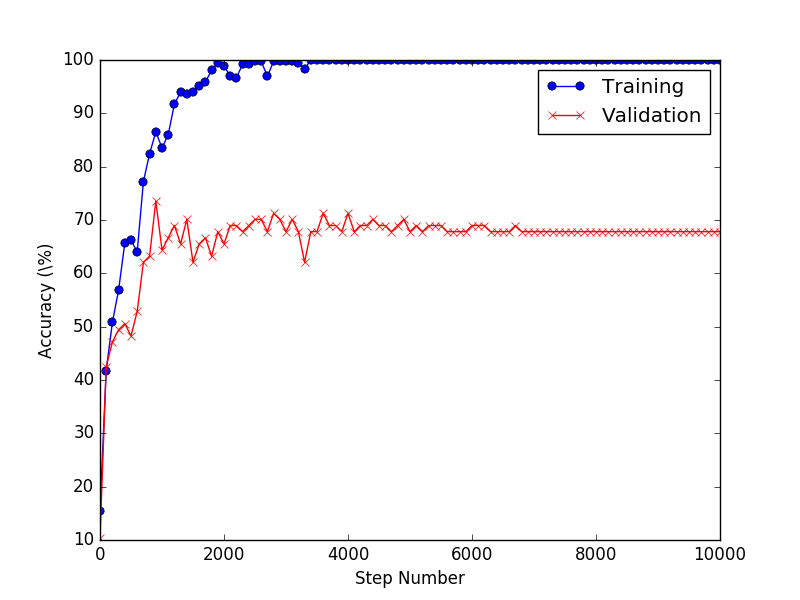
\includegraphics [trim=0 0 0 0, clip, angle=0, width=0.8\columnwidth,
	keepaspectratio]{figures/2_3_num_steps}
	\caption{Training and validation accuracy are plotted over 10,000 training steps. Validation performance levels off after 1,000 training steps, but training accuracy continues to increase. This behavior looks like overfitting, so training should be stopped early around step 1,000.} 
	\label{fig:2_3_num_steps} 
\end{figure}

The pooling layers seem to make no difference on performance.

\subsection{Part 4}
Finally, we use the network on a transformed version of the dataset.
Results in \cref{table_2_4} show that the performance is not the same for every transormation type.
For example, the original CNN only gets 10\% accuracy on inverted images, compared to 66.7\% on low contrast images (all relative to a 70.1\% accuracy on normal images).

\cref{table_2_4}'s columns show the original CNN, a CNN with Early Stopping and one with both Early Stopping and Max Pooling.
The results are not significantly different.
This aligns with the earlier observation that max pooling does not affect this problem much.
Early Stopping surprisingly didn't have much effect either.


\begin{table}[ht!]
\centering
\begin{tabular}{||c c c c||}  
 \hline
  & Regular & ES & ES \& Pooling \\
 Transformation & Val Acc (\%) & Val Acc (\%) & Val Acc (\%) \\ [0.3ex] 
 \hline\hline
 Normal & 65.5 & 70.1 & 69.0 \\ \hline
 Translated & 33.3 & 29.9 & 35.6 \\ \hline
 Brightened & 46.0 & 47.1 & 43.7 \\ \hline
 Darkened & 47.1 & 49.4 & 46.0 \\ \hline
 High Contrast & 62.1 & 63.2 & 58.6 \\ \hline
 Low Contrast & 66.7 & 66.7 & 67.8 \\ \hline
 Flipped & 42.5 & 41.4 & 44.8 \\ \hline
 Inverted & 8.0 & 10.3 & 12.6 \\ \hline
\end{tabular}
\caption{Accuracy of CNNs on transformed dataset, with Early Stopping (ES) and Max pooling.}
\label{table_2_4}
\end{table}




\section{Pegasos} \label{sec:prob3}
In this section, we use the Pegasos algorithm for soft-margin SVM binary classification of one of the 2D datasets.

\subsection{Part 1}
The Pegasos algorithm is a method to solve soft-margin SVM.
We implemented the algorithm according to the provided pseudocode, and added a bias term, $w_0$ that is incremented by $\eta_ty_i$ for misclassified sample $x_i$ each iteration.
The bias term is not penalized by the regularization.
The formulation solved by Pegasos is:
\begin{equation}\label{eq:svm_pegasos}
min_w \frac{\lambda}{2}||w||^2 + \frac{1}{N}\sum\limits_{i=1}^{N}max\{0,1-y_i(w^Tx_i)\}
\end{equation}

\subsection{Part 2}
The algorithm is applied to the same 2D dataset for several values of $\lambda$ ($\lambda = [2, 2^{-1}, 2^{-2}, 2^{-4}$), shown in~\cref{fig:3_2_lambdas}.
For large $\lambda$ (left), magnitude of $w$ is penalized heavily, so the decision boundary is not very accurate.
As $\lambda$ decreases, the regularization penalty becomes less dominant compared with accuracy, so the accuracy improves.
This intuition agrees with the objective function~\cref{eq:svm_pegasos}.

\begin{figure}
	\centering
	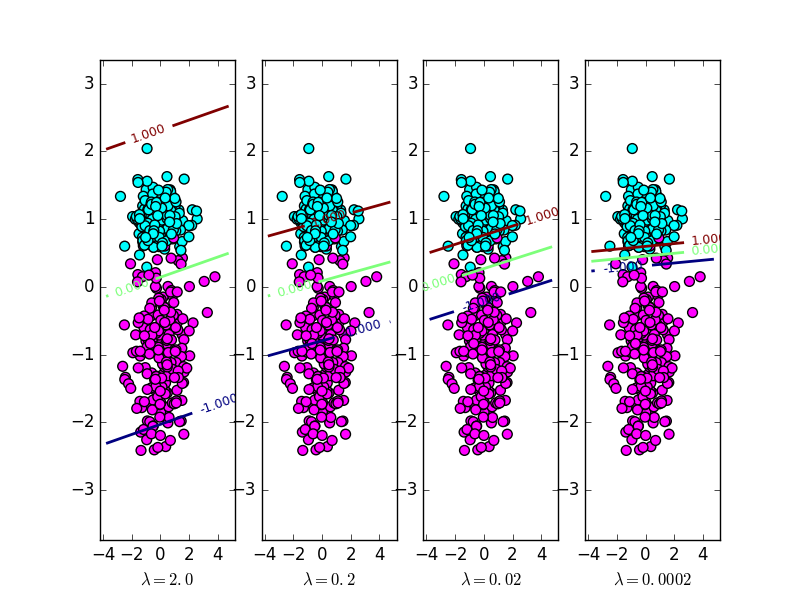
\includegraphics [trim=0 0 0 0, clip, angle=0, width=0.8\columnwidth,
	keepaspectratio]{figures/3_2_lambdas}
	\caption{The Pegasos algorithm is applied to the same dataset with four different regularization parameter values, $\lambda$. For large $\lambda$ (left), magnitude of $w$ is penalized heavily, so the decision boundary is not very accurate. As $\lambda$ decreases, the regularization penalty becomes less dominant compared with accuracy, so the accuracy improves.}
	\label{fig:3_2_lambdas} 
\end{figure}

\subsection{Part 3}
Next, we extended our implementation to handle a kernel matrix input, and tested it with a gaussian RBF kernel as in~\cref{sec:prob2}.
After learning $\alpha$, we predict the class of a new sample, $x_i$ by first calculating $c = \alpha \cdot K(X, x_i; \gamma)$, where $X$ is the entire training set and $\gamma$ is the Gaussian kernel bandwidth.
If $c > 0$, it's part of the positive class, otherwise it's the negative class.

\subsection{Part 4}
We tested our algorithm on multiple values of $\gamma$ with a fixed $\lambda=0.02$.
For large $\gamma$ (left), [todo], and the decision boundary overfits the data, evident in the decision boundary's jagged shape tracing around individual borderline samples.
As $\gamma$ decreases, the accuracy decreases, but the decision boundary is much less complicated.
This usually leads to better generalization to unseen data.

The number of support vectors decreases as $\gamma$ increases (192, 165, 10, 22).
This observation aligns with the decreasing complexity of the decision boundary, because each support vector affects the shape of the decision boundary.

These observations associated with increasing $\gamma$ match the trends seen in~\cref{sec:prob2} with increasing $C$.
Both implementations (Pegasos and SVM) are able to correctly classify the dataset.
Our Pegasos implementation runs much faster, making it easier to test with different parameters for increased performance.


\begin{figure}
	\centering
	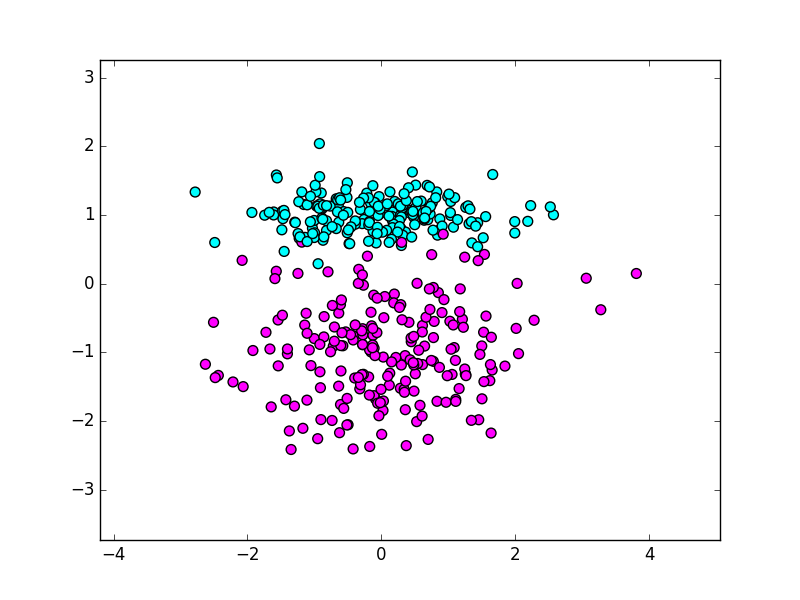
\includegraphics [trim=0 0 0 0, clip, angle=0, width=0.8\columnwidth,
	keepaspectratio]{figures/3_3_decisions}
	\caption{The Pegasos algorithm is applied to the same dataset with four different kernel bandwidth values, $\gamma = [2^2, 2^1, 2^0, 2^{-1}]$. For large $\gamma$ (left), [todo], and the decision boundary overfits the data. As $\gamma$ decreases, the accuracy decreases, but the decision boundary is much less complicated.}
	\label{fig:3_3_decisions} 
\end{figure}
%\listofchanges

%\balance

% \addtolength{\textheight}{-12cm} % This command serves to balance the column lengths
% on the last page of the document manually. It shortens
% the textheight of the last page by a suitable amount.
% This command does not take effect until the next page
% so it should come on the page before the last. Make
% sure that you do not shorten the textheight too much.

%%%%%%%%%%%%%%%%%%%%%%%%%%%%%%%%%%%%%%%%%%%%%%%%%%%%%%%%%%%%%%%%%%%%%%%%%%%%%%%%



%%%%%%%%%%%%%%%%%%%%%%%%%%%%%%%%%%%%%%%%%%%%%%%%%%%%%%%%%%%%%%%%%%%%%%%%%%%%%%%%



%%%%%%%%%%%%%%%%%%%%%%%%%%%%%%%%%%%%%%%%%%%%%%%%%%%%%%%%%%%%%%%%%%%%%%%%%%%%%%%%
% \section*{Acknowledgment}
% This work is supported by Ford Motor Company.
%%%%%%%%%%%%%%%%%%%%%%%%%%%%%%%%%%%%%%%%%%%%%%%%%%%%%%%%%%%%%%%%%%%%%%%%%%%%%%%%
%\clearpage
\balance
% \bibliographystyle{IEEEtran} 
% %\bibliographystyle{unsrt} 
% \bibliography{biblio}
% %\balance
\end{document}
%\grid
